% Created by tikzDevice version 0.12 on 2019-02-23 16:14:03
% !TEX encoding = UTF-8 Unicode
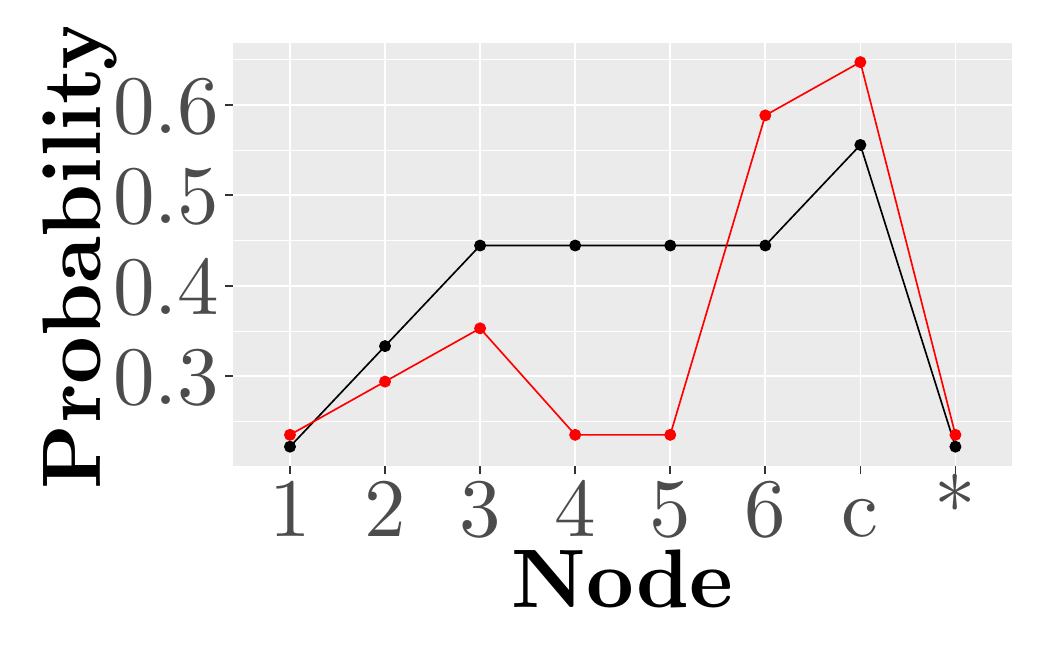
\begin{tikzpicture}[x=1pt,y=1pt]
\definecolor{fillColor}{RGB}{255,255,255}
\path[use as bounding box,fill=fillColor,fill opacity=0.00] (0,0) rectangle (361.35,216.81);
\begin{scope}
\path[clip] (  0.00,  0.00) rectangle (361.35,216.81);
\definecolor{drawColor}{RGB}{255,255,255}
\definecolor{fillColor}{RGB}{255,255,255}

\path[draw=drawColor,line width= 0.6pt,line join=round,line cap=round,fill=fillColor] (  0.00,  0.00) rectangle (361.35,216.81);
\end{scope}
\begin{scope}
\path[clip] ( 74.17, 58.45) rectangle (355.85,211.31);
\definecolor{fillColor}{gray}{0.92}

\path[fill=fillColor] ( 74.17, 58.45) rectangle (355.85,211.31);
\definecolor{drawColor}{RGB}{255,255,255}

\path[draw=drawColor,line width= 0.3pt,line join=round] ( 74.17, 74.49) --
	(355.85, 74.49);

\path[draw=drawColor,line width= 0.3pt,line join=round] ( 74.17,107.20) --
	(355.85,107.20);

\path[draw=drawColor,line width= 0.3pt,line join=round] ( 74.17,139.91) --
	(355.85,139.91);

\path[draw=drawColor,line width= 0.3pt,line join=round] ( 74.17,172.61) --
	(355.85,172.61);

\path[draw=drawColor,line width= 0.3pt,line join=round] ( 74.17,205.32) --
	(355.85,205.32);

\path[draw=drawColor,line width= 0.6pt,line join=round] ( 74.17, 90.84) --
	(355.85, 90.84);

\path[draw=drawColor,line width= 0.6pt,line join=round] ( 74.17,123.55) --
	(355.85,123.55);

\path[draw=drawColor,line width= 0.6pt,line join=round] ( 74.17,156.26) --
	(355.85,156.26);

\path[draw=drawColor,line width= 0.6pt,line join=round] ( 74.17,188.97) --
	(355.85,188.97);

\path[draw=drawColor,line width= 0.6pt,line join=round] ( 94.78, 58.45) --
	( 94.78,211.31);

\path[draw=drawColor,line width= 0.6pt,line join=round] (129.13, 58.45) --
	(129.13,211.31);

\path[draw=drawColor,line width= 0.6pt,line join=round] (163.48, 58.45) --
	(163.48,211.31);

\path[draw=drawColor,line width= 0.6pt,line join=round] (197.84, 58.45) --
	(197.84,211.31);

\path[draw=drawColor,line width= 0.6pt,line join=round] (232.19, 58.45) --
	(232.19,211.31);

\path[draw=drawColor,line width= 0.6pt,line join=round] (266.54, 58.45) --
	(266.54,211.31);

\path[draw=drawColor,line width= 0.6pt,line join=round] (300.89, 58.45) --
	(300.89,211.31);

\path[draw=drawColor,line width= 0.6pt,line join=round] (335.24, 58.45) --
	(335.24,211.31);
\definecolor{drawColor}{RGB}{0,0,0}
\definecolor{fillColor}{RGB}{0,0,0}

\path[draw=drawColor,line width= 0.4pt,line join=round,line cap=round,fill=fillColor] ( 94.78, 65.40) circle (  1.96);

\path[draw=drawColor,line width= 0.4pt,line join=round,line cap=round,fill=fillColor] (129.13,101.74) circle (  1.96);

\path[draw=drawColor,line width= 0.4pt,line join=round,line cap=round,fill=fillColor] (163.48,138.09) circle (  1.96);

\path[draw=drawColor,line width= 0.4pt,line join=round,line cap=round,fill=fillColor] (197.84,138.09) circle (  1.96);

\path[draw=drawColor,line width= 0.4pt,line join=round,line cap=round,fill=fillColor] (232.19,138.09) circle (  1.96);

\path[draw=drawColor,line width= 0.4pt,line join=round,line cap=round,fill=fillColor] (266.54,138.09) circle (  1.96);

\path[draw=drawColor,line width= 0.4pt,line join=round,line cap=round,fill=fillColor] (300.89,174.43) circle (  1.96);

\path[draw=drawColor,line width= 0.4pt,line join=round,line cap=round,fill=fillColor] (335.24, 65.40) circle (  1.96);

\path[draw=drawColor,line width= 0.6pt,line join=round] ( 94.78, 65.40) --
	(129.13,101.74) --
	(163.48,138.09) --
	(197.84,138.09) --
	(232.19,138.09) --
	(266.54,138.09) --
	(300.89,174.43) --
	(335.24, 65.40);
\definecolor{drawColor}{RGB}{255,0,0}
\definecolor{fillColor}{RGB}{255,0,0}

\path[draw=drawColor,line width= 0.4pt,line join=round,line cap=round,fill=fillColor] ( 94.78, 69.68) circle (  1.96);

\path[draw=drawColor,line width= 0.4pt,line join=round,line cap=round,fill=fillColor] (129.13, 88.92) circle (  1.96);

\path[draw=drawColor,line width= 0.4pt,line join=round,line cap=round,fill=fillColor] (163.48,108.16) circle (  1.96);

\path[draw=drawColor,line width= 0.4pt,line join=round,line cap=round,fill=fillColor] (197.84, 69.68) circle (  1.96);

\path[draw=drawColor,line width= 0.4pt,line join=round,line cap=round,fill=fillColor] (232.19, 69.68) circle (  1.96);

\path[draw=drawColor,line width= 0.4pt,line join=round,line cap=round,fill=fillColor] (266.54,185.12) circle (  1.96);

\path[draw=drawColor,line width= 0.4pt,line join=round,line cap=round,fill=fillColor] (300.89,204.36) circle (  1.96);

\path[draw=drawColor,line width= 0.4pt,line join=round,line cap=round,fill=fillColor] (335.24, 69.68) circle (  1.96);

\path[draw=drawColor,line width= 0.6pt,line join=round] ( 94.78, 69.68) --
	(129.13, 88.92) --
	(163.48,108.16) --
	(197.84, 69.68) --
	(232.19, 69.68) --
	(266.54,185.12) --
	(300.89,204.36) --
	(335.24, 69.68);
\end{scope}
\begin{scope}
\path[clip] (  0.00,  0.00) rectangle (361.35,216.81);
\definecolor{drawColor}{gray}{0.30}

\node[text=drawColor,anchor=base east,inner sep=0pt, outer sep=0pt, scale=  3.00] at ( 69.22, 80.51) {0.3};

\node[text=drawColor,anchor=base east,inner sep=0pt, outer sep=0pt, scale=  3.00] at ( 69.22,113.22) {0.4};

\node[text=drawColor,anchor=base east,inner sep=0pt, outer sep=0pt, scale=  3.00] at ( 69.22,145.93) {0.5};

\node[text=drawColor,anchor=base east,inner sep=0pt, outer sep=0pt, scale=  3.00] at ( 69.22,178.64) {0.6};
\end{scope}
\begin{scope}
\path[clip] (  0.00,  0.00) rectangle (361.35,216.81);
\definecolor{drawColor}{gray}{0.20}

\path[draw=drawColor,line width= 0.6pt,line join=round] ( 71.42, 90.84) --
	( 74.17, 90.84);

\path[draw=drawColor,line width= 0.6pt,line join=round] ( 71.42,123.55) --
	( 74.17,123.55);

\path[draw=drawColor,line width= 0.6pt,line join=round] ( 71.42,156.26) --
	( 74.17,156.26);

\path[draw=drawColor,line width= 0.6pt,line join=round] ( 71.42,188.97) --
	( 74.17,188.97);
\end{scope}
\begin{scope}
\path[clip] (  0.00,  0.00) rectangle (361.35,216.81);
\definecolor{drawColor}{gray}{0.20}

\path[draw=drawColor,line width= 0.6pt,line join=round] ( 94.78, 55.70) --
	( 94.78, 58.45);

\path[draw=drawColor,line width= 0.6pt,line join=round] (129.13, 55.70) --
	(129.13, 58.45);

\path[draw=drawColor,line width= 0.6pt,line join=round] (163.48, 55.70) --
	(163.48, 58.45);

\path[draw=drawColor,line width= 0.6pt,line join=round] (197.84, 55.70) --
	(197.84, 58.45);

\path[draw=drawColor,line width= 0.6pt,line join=round] (232.19, 55.70) --
	(232.19, 58.45);

\path[draw=drawColor,line width= 0.6pt,line join=round] (266.54, 55.70) --
	(266.54, 58.45);

\path[draw=drawColor,line width= 0.6pt,line join=round] (300.89, 55.70) --
	(300.89, 58.45);

\path[draw=drawColor,line width= 0.6pt,line join=round] (335.24, 55.70) --
	(335.24, 58.45);
\end{scope}
\begin{scope}
\path[clip] (  0.00,  0.00) rectangle (361.35,216.81);
\definecolor{drawColor}{gray}{0.30}

\node[text=drawColor,anchor=base,inner sep=0pt, outer sep=0pt, scale=  3.00] at ( 94.78, 32.84) {1};

\node[text=drawColor,anchor=base,inner sep=0pt, outer sep=0pt, scale=  3.00] at (129.13, 32.84) {2};

\node[text=drawColor,anchor=base,inner sep=0pt, outer sep=0pt, scale=  3.00] at (163.48, 32.84) {3};

\node[text=drawColor,anchor=base,inner sep=0pt, outer sep=0pt, scale=  3.00] at (197.84, 32.84) {4};

\node[text=drawColor,anchor=base,inner sep=0pt, outer sep=0pt, scale=  3.00] at (232.19, 32.84) {5};

\node[text=drawColor,anchor=base,inner sep=0pt, outer sep=0pt, scale=  3.00] at (266.54, 32.84) {6};

\node[text=drawColor,anchor=base,inner sep=0pt, outer sep=0pt, scale=  3.00] at (300.89, 32.84) {c};

\node[text=drawColor,anchor=base,inner sep=0pt, outer sep=0pt, scale=  3.00] at (335.24, 32.84) {*};
\end{scope}
\begin{scope}
\path[clip] (  0.00,  0.00) rectangle (361.35,216.81);
\definecolor{drawColor}{RGB}{0,0,0}

\node[text=drawColor,anchor=base,inner sep=0pt, outer sep=0pt, scale=  3.00] at (215.01,  7.44) {\bfseries Node};
\end{scope}
\begin{scope}
\path[clip] (  0.00,  0.00) rectangle (361.35,216.81);
\definecolor{drawColor}{RGB}{0,0,0}

\node[text=drawColor,rotate= 90.00,anchor=base,inner sep=0pt, outer sep=0pt, scale=  3.00] at ( 26.20,134.88) {\bfseries Probability};
\end{scope}
\end{tikzpicture}
